\section{Methods}

\subsection{Notation}

\subsection{Models of BEM}
The motivation of BEM originates from the cognitive science. Human beings's understanding process works in two systems: (System I) unconsciously retrieves pieces of knowledge associated with the given task; (System II) subjectively use analytic reasoning to analyze or ponder the received information. In spirit, the triplets in the knowledge graph function and distribute similarly to the knowledge used in System I: they provide association rather than causlity; they are scattered around rather than organized. Therefore, we are motivated to design a model that mimics System II. The triplets in the knowledge graph are regarded as the base knowledge that will be further processed to solve a specific task. In other words, the embedding from the knowledge graph should be corrected in terms of the task to tackle.

We first start with the simplest case where each entity has two embeddings, one from the knowledge graph and the other given by a specific task. For an entity $e$, we suppose that the task-specific embedding $\bz_{e}$ is generated from a distribution determined by the knowledge graph embedding  $\bh_{e}$ and a correction term with $\bdelta_e$ respect to the task, that is,
\begin{equation}
  \bz_{e} \approx \bff(\bh_e + \bdelta_e),
  \label{eq:connection_z_h_1st}
\end{equation}
where $\bff$ is a non-linear function that projects $\bh_e + \bdelta_e$ as $\bz_e$. However, both $\bz_e$ and $\bh_e$ are distributed on the sphere. The set of all $\bz_{e}'s$ (or $\bh_{e}'s$) is the same for the downstream goal such as classification or prediction, up to a variety of operations including rotation and reflection. A sufficiently complicated non-linear function $\bff$ is required to express such operation. However, the number of parameters are obviously larger than the sample size, since each entity needs a correction term. Learning $\bdelta_e$'s and $\bff$ seems infeasible. On the other hand, we note that the learnings of both the knowledge graph embeddings and the task-specific embeddings are highly dependent on the interaction between entities. Decoupling the second-order information between entities as \eqref{eq:connection_z_h_1st} might lead to an intolerable loss regarding the goal for a good embedding. Considering the interaction not only retains the loss of key information, but also increases the sample sizes (there are $N_e^2$ pairs of entities). With these considerations, we formulate a generation model from $\bh_e$ to $\bz_e$:
\begin{itemize}
\item [1.] For each entity $e$:
  \begin{itemize}
	\item sample its correction variable $\bdelta_e \sim N(\bold 0, \lambda_1 \cdot s_h^2)$, where $\lambda_1$ is a tuning parameter and $s_h^2$ is estimated by $\bold h_e$.
	\item sample its assoiated uncertainty variable $\bsigma_{e_j}^2 \sim \text{log~Normal}(\ell_{\mu_e}, \lambda_2\cdot \ell_{\sigma^2_e})$, where $j = 1, \ldots, d_2$. Here, $\ell_{\mu_e}$, $\ell_{\sigma^2_e}$ can be estimated by $\bold z_e$'s, and $\lambda_2$ is a tuning parameter.
      \end{itemize}
    \item [2.] For each pair of entities, $e_1$, $e_2$, sample
      \begin{equation}
        \bold z_{e_1} - \bold z_{e_2} \sim  N\left ( \bff_{\phi}(\bh_{e_1} +  \bdelta_{e_1}) - \bff_{\phi}(\bh_{e_2} + \bdelta_{e_2}), \text{diag}(\bsigma_{e_1}^2 + \bsigma_{e_2}^2) \right),
        \label{eq:connection_z_h_2nd}
        \end{equation}
where $\bff_{\phi}$ is a neural network with parameter $\phi$. 
\end{itemize}
The model is depicted in Figure \ref{fig:generation_model} as well. Our goal is to seek the best parameter $\phi$ and the posteriors of $\bdelta_e$'s, $\bsigma_{e_j}$'s in \eqref{eq:connection_z_h_2nd}, given all the $\bh_e$'s and $\bz_e$'s. Suppose the fitted network paramter is $\hat{\phi}$ and the posterior mean of $\bdelta_e$ is $\hat{\bmu}_{e}$, we use $\bh_e +\hat{\bmu}_{e}$ as the corrected embedding for the knowledge graph, and $\bff_{\hat{\phi}}(\bh_e +\hat{\bmu}_{e})$ as the corrected embedding for the specific task.

\begin{figure}[h]
  \centering
  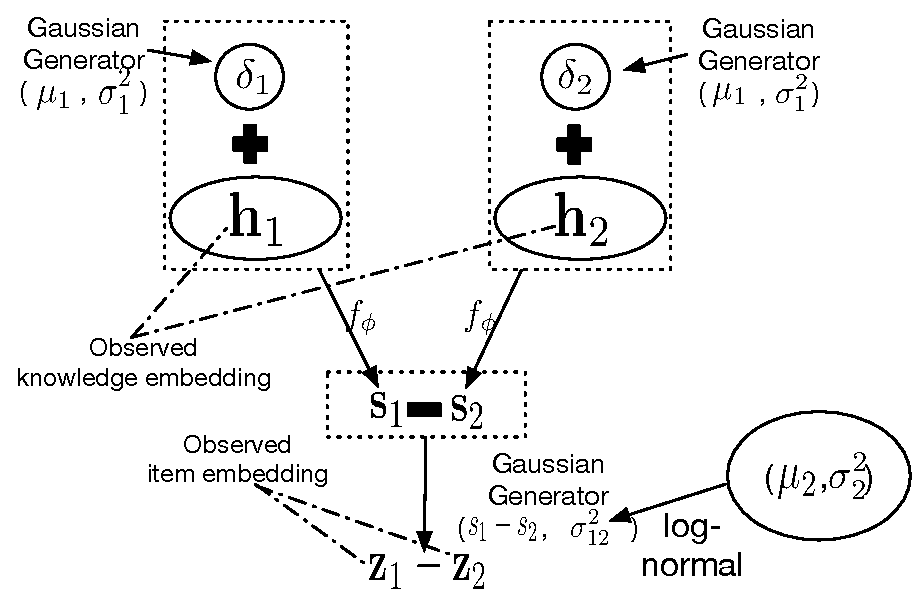
\includegraphics[width=0.5\textwidth]{./fig/generation.pdf}
  \caption{The BEM model.}
  \label{fig:generation_model}
\end{figure}
\subsection{Algorithm of BEM}

